\chapter{Inleiding}
Een aanbevelingssysteem is een handig middel om zich een weg te banen doorheen de enorme hoeveelheid content die sommige webapplicaties aanbieden. Het laat ons toe snel interessante en persoonsgerichte items te vinden.
Aanbevelingssystemen kunnen mensen nieuwe vrienden leren kennen of zorgen voor een boost in verkoopcijfers door gerichte marketing. Ze kunnen ook gebruikt worden om de gebruiker nieuwe dingen aan te leren. Zo zal bijvoorbeeld OWL \cite{Linton00owl} gebruikers nieuwe shortcuts aanreiken voor veelgebruikte commando's in een bepaald programma. Het kan ook een doel zijn om een community van gebruikers te cre\"eren rond items. Een voorbeeld hiervan is Tripadvisor.com, waar men niet beoogt om zoveel mogelijk reservaties te verkrijgen maar eerder een community uit te bouwen die elkaar helpt bij het kiezen tussen hotels. 
Service providers die klassieke aanbevelingssystemen gebruiken houden vaak veel persoonlijke data bij op hun servers. De data van een persoon wordt bijgehouden in zijn gebruikersprofiel. Google heeft al aangegeven dat het alle data van \'e\'en persoon van zijn verschillende services bijhoudt in \'e\'en profiel. 

Het bijhouden van deze gigantische hoeveelheden data brengt vragen met zich mee:
\begin{itemize}
 
\item Wordt deze data wel correct beheerd? 
\item Welke risico's zijn er voor onze privacy?
\item Kan misbruik vermeden worden met alternatieve privacyvriendelijkere methodes?
\end{itemize}

Aanbevelingen zijn logischerwijs gezien beter of nauwkeuriger naarmate het systeem beschikt over meer gedetailleerde data. Er is dus in zekere zin een inherente wisselwerking tussen de privacy van de gebruiker en de nauwkeurigheid van het systeem. In deze masterproef concentreren we ons op hoe we de verschillende klassieke algoritmes om aanbevelingen te berekenen kunnen aanpassen zodat er minder risico is op privacy-inbreuken in verband met persoonlijke voorkeuren of persoonlijke informatie in het algemeen. Jammer genoeg hebben de mogelijkheden die al beschreven zijn in de literatuur een negatieve impact op de systeemprestatie en/of de nauwkeurigheid van de aanbevelingen. 
\begin{figure}[htpb]   
    \label{Figuur::wisselwerking}      
  \begin{center}    
 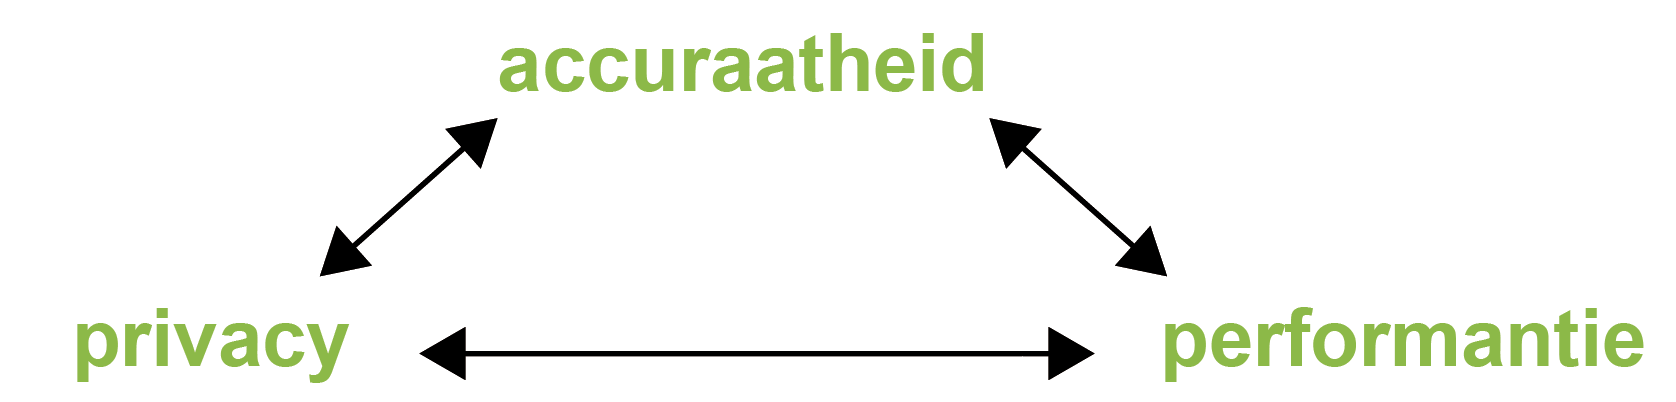
\includegraphics[width=\textwidth,height=\textheight,keepaspectratio]{fig/wisselwerking}    
  \end{center}     
   \end{figure}\\
Het doel van deze masterproef is een optimale oplossing te vinden voor deze drievoudige wisselwerking en dus het algoritme te vinden dat enerzijds privacyvriendelijk is maar waarvan anderzijds het prestatieniveau aanvaardbaar is en de aanbevelingen goed en persoonsgericht zijn. Ook wordt er rekening gehouden met de mobiele setting: het algoritme moet bruikbaar zijn op een smartphone en dus rekening houden met beperkingen zoals rekenkracht en batterijgebruik.\\

Hiervoor bekijken we in hoofdstuk \ref{privacyklassiek} in paragraaf \ref{sec:klassiek} de klassieke aanbevelingssystemen en welke privacygevoelige data deze bijhouden. Vervolgens beschouwen we in paragrafen \ref{sec:privacy} tot en met \ref{sec:risicos} de betekenis van privacy in de context van een aanbevelingssysteem en de risico's die voorkomen bij bestaande aanbevelingssystemen. In hoofdstuk \ref{onderzoek} worden de bestaande oplossingen bestudeerd en geanalyseerd en bekeken welke het best scoort op de drie hoofdpunten, rekening houdend met een mobiele setting. De beste optie wordt als vertrekpunt genomen voor de uitwerking van een werkend privacyvriendelijk aanbevelingssysteem in hoofdstuk \ref{privacy_opl}. We kozen aan de client-kant voor een Androidapplicatie en aan de kant van de server kozen we voor Java.
 
